\newpage
\section{Parabole}

\subsection{Définition focale}\label{section:paramonofo}
Contrairement à l'ellipse et l'hyperbole, la parabole ne possède pas de définition bifocale puisqu'elle ne possède qu'un foyer.
Repartons de la définition focale des coniques \ref{def:conique_mono}.

\begin{tcolorbox}[colback=cyan!5, colframe=cyan!70!blue, title=Définition focale d'une parabole]
\defn{Soit $F$, un point du plan $\Pi$.\\
Une parabole de foyer $F$ est le lieu des points $M $ du plan $\Pi$ tels que la distance de $M$ à au foyer $F$ est égale à la distance de $M$ à une droite directrice $d_F$.

}\label{def:para_mono}
\begin{equation}
    \mathcal{P} \equiv \left\{ M \in \Pi \;\big\vert\; d(M,F) = d(M,d_F) \right\}
\end{equation}

L'\textbf{excentricité} vaut 1.\\
La distance entre le foyer $F$ et la directrice $d_F$ est appelée \textbf{paramètre}, $d(F,d_F) = p >0$.\\
\end{tcolorbox}

\begin{figure}[H]
    \centering
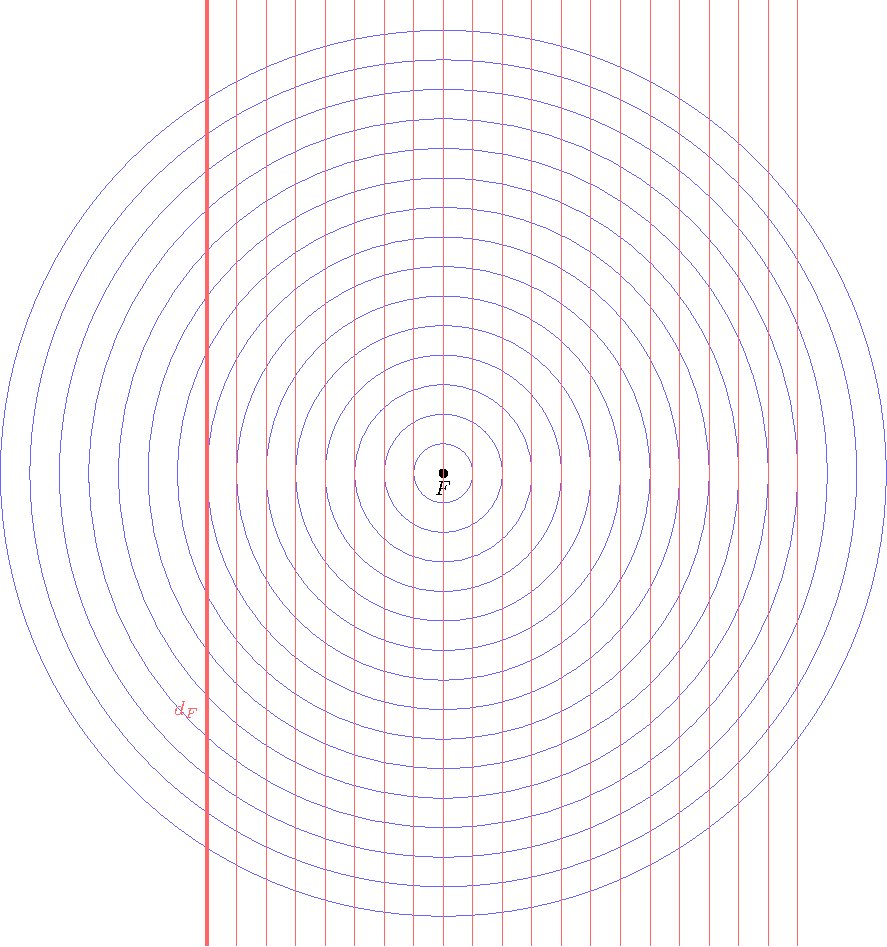
\includegraphics[scale = 0.8]{sections/tikz_standalone/para_1.pdf}
\end{figure}
\normalfont
A partir de cette définition, tracez une parabole. Que vaut le paramètre $p$ ?\\
Sans guide tracé, sauriez-vous le refaire avec un compas et une latte ?
\newpage
\null
\newpage
\null
\newpage
%DEMO
\null
\newpage
\null
\newpage
\null
\newpage
%Exemples
\null
\newpage
\null
\newpage
\null
\newpage

\subsection{Etude fonctionnelle et graphique}\label{section:paragrap}
\newpage
\null
\newpage
